%%%%%%%%%%%%%%%%%%%%%%%%%%%%%%%%%%%%%%%%%%%%%%%%%%%%%%%%%%%%%%%%%%%%%%
%
% レポートテンプレート
%
% updated 22 Oct, 2018
% last updated 02 April, 2019
%
% 各自のレポートに合わせて変更して使ってください.上記の行は残して使うこと.

%%%%%%%%%%%%%%%%%%%%%%%%%%%%%%%%%%%%%%%%%%%%%%%%%%%%%%%%%%%%%%%%%%%%%%
\documentclass[a4paper,10pt]{jarticle}
\usepackage[dvipdfmx]{graphicx}
\usepackage{amsmath}
\usepackage{latexsym}
\usepackage{multirow}
\usepackage{url}
\setlength{\textwidth}{165mm} %165mm-
\setlength{\marginparwidth}{40mm}
\setlength{\textheight}{225mm}
\setlength{\topmargin}{-5mm}
\setlength{\oddsidemargin}{-3.5mm}

\def\vector#1{\mbox{\boldmath $#1$}}
\newcommand{\AmSLaTeX}{%
 $\mathcal A$\lower.4ex\hbox{$\!\mathcal M\!$}$\mathcal S$-\LaTeX}
\newcommand{\PS}{{\scshape Post\-Script}}
\def\BibTeX{{\rmfamily B\kern-.05em{\scshape i\kern-.025em b}\kern-.08em
 T\kern-.1667em\lower.7ex\hbox{E}\kern-.125em X}}
\newcommand{\pderiv}[2]{{\partial#1\over\partial#2}}
\newcommand{\DeLta}{{\mit\Delta}}
\renewcommand{\d}{{\rm d}}
\def\wcaption#1{\caption[]{\parbox[t]{100mm}{#1}}}
\def\rm#1{\mathrm{#1}}
\def\tempC{^\circ \rm{C}}


%%%%%%%%%%%%%%%%%%%%%%%%%%%%%%%%%%%%%%%%%%%%%%%%%%%%%%%%%%%%%%%%%%%%%%
\begin{document}
%
\begin{center}
{\Large{\bf 光のスペクトルに関するレポート}} \\
{\bf 電気通信大学 1類1クラス\\
2311009 アハメドアティフ} \\
{\bf 2023年5月22日作成} \\
{\bf 2023年5月25日更新}
\end{center}
%%%%%%%%%%%%%%%%%%%%%%%%%%%%%%%%%%%%%%%%%%%%%%%%%%%%%%%%%%%%%%%%%%%%%%
\section{目的}

 実験の目的は、光源NaランプやHランプを用い、回折格子分光計を使ってそれぞれの原子に
特有なスペクトル線を観測し、その波長を求めるためにまず回折格子の格子定数を求める測定
をして、その求めた値を用いて原子のスペクトル線の波長を求め、不確かさを求めたうえで
理科年表に載っている値と実験地を比較した上で、光の色と波長の関係を調べることである。

%%%%%%%%%%%%%%%%%%%%%%%%%%%%%%%%%%%%%%%%%%%%%%%%%%%%%%%%%%%%%%%%%%%%%%
\section{原理}
 スリットを狭い間隔で平行に並べたものを回折格子という。特定の波長の単色な平行光線を
回折格子の面に垂直に当てると、回折格子を通った光はいくつかの方向に現れる。入射方向に出てくる光線を
0次、それより角度の増す方向に順次一次、二次、…の回折光という。入射光の方向と回折光の方向のなす角を
回折角という。$m$次回折光の回折角 $\theta_m$ は次の式で与えられる。


\begin{equation}
d\sin\theta_m = m\randa  または  \ramda=\frac{\sin\theta_m}{mN}
\label{grav_eq}
\end{equation}

 ここで$\ramda$は光の波長、$d$は回折格子の間隔("格子間隔"  または  "格子定数")、
$N$は$d$の逆数で単位長さ当たりの格子の数である。回折格子の特性を表すときにはdよりも
$N$を用いる。式(\ref{grav_eq})は、隣接するスリットを通った光が強めあう条件を示したものであり、
光路差$d$$\sin\theta$が波長の整数倍に等しいことを示している。いろいろな波長を含む光を
回折格子に当てると回折光はいくつかの方向に分かれて回折し、入射した光のスペクトルが観測される。
スペクトル線には次数$m$が同じ回折光を比べると波長の長い赤いスペクトル線の方が波長の短い
青いスペクトル線より回折角が大きい性質がある。すなわち、$N$が既知なら回折角を測れば波長を求めることができる。

\vspace{3mm}

%
\subsection{重力加速度の測定}
不確かさを求める式は次のようになります.
\begin{eqnarray}
\overline{g}=\cfrac{\cfrac{g_1}{(\Delta g_1)^2}+\cfrac{g_2}{(\Delta g_2)^2}+\cdots+\cfrac{g_n}{(\Delta g_n)^2}}{\cfrac{1}{(\Delta g_1)^2}+\cfrac{1}{(\Delta g_2)^2}+\cdots+\cfrac{1}{(\Delta g_n)^2}} \\
\label{eq1}
\Delta g = \cfrac{1}{\sqrt{\cfrac{1}{(\Delta g_1)^2}+\cfrac{1}{(\Delta g_2)^2}+\cdots+\cfrac{1}{(\Delta g_n)^2}}}
\label{eq2}
\end{eqnarray}

%

\subsection{光のスペクトル}
Na線の D$_1$線とD$_2$線の波長.

 D$_1$線:589.592 nm \\
 
 ${\rm D_2}$線:588.995 $\rm{nm}$

 \vspace{2mm}
 上記は同じ表示になるものを異なる方法で表記しています.ただし\verb|\rm|のコマンドは
 このファイルの冒頭で再定義しており,\TeX の本来のコマンドとは異なる挙動をしています.

%%%%%%%%%%%%%%%%%%%%%%%%%%%%%%%%%%%%%%%%%%%%%%%%%%%%%%%%%%%%%%%%%%%%%%
\section{方法}

\subsection{実験器具}

 光学系(コリメーター、回折格子、望遠鏡から成る)、Na管、H管、Hg管,衝立

ここで装置の概略図を図(\ref{spk})に掲載する。R$_1$はピント調整ネジを示している。

\begin{figure}[ht]
\begin{center}
\includegraphics*[scale=1.0]{spk.png}
\caption{実験の概略図}
\label[spk]
\end{center}
\end{figure}
\subsection{実験方法}
 
%

 実験方法は、まず望遠鏡固定ネジを緩めて、目盛盤固定ネジを硬く締めて、望遠鏡を覗き、
レンズの十字線がはっきり見えるように望遠鏡の接眼レンズを前後に動かし、ピントを合わせる。
次に望遠鏡を除いた時に下部に見えるスリットの輪郭がはっきり見えるように伸縮ネジを動かしピントを合わせる。
この操作をしないとスリットの像と十字線が重ならないため視差が残るため重要である。回折格子は精密かつ繊細な
光学素子であるため、くれぐれも表面に指紋をつけることのないように注意して、コリメーターと
望遠鏡の間にある回転台にのせて、上方から見て回折格子の格子面をコリメーターの軸と可能な限り垂直になるように
回転台を回す
その作業が終わったらスペクトルの管をスターターにつけて、スターターの電源をONにしてスタートボタンを暫く押し続けて、
スペクトル管のフィラメントが赤熱してきたらボタンから手を離す。そしてコリメーターのスリットにつく寸前までスペクトル管を近づける。
そしたら、実験室の照明を消してなるべくスペクトル管の光以外の光が入り込まないように衝立を立てる。
ここまでいってから望遠鏡を覗いてスペクトルの観察をし、分光器のメモリを測定する。この時スペクトルについては望遠鏡の
初期位置を基準に、その左右でそれぞれ第一次回折光と第二次回折光、また見えれば第三次回折光の角度を目盛盤で測った。
実験では二種類の課題を行っている。

 一つ目の課題はNa管を用いた測定で、はじめからNa管のスペクトルのうちのD$_1$線とD$_2$次線の
波長は与えられていて、その波長の値と分光器での測定によって求めた角度を以下の式(\ref{grav2_eq})に代入して求めた
角度$\theta_m$を式(\ref{grav_eq})に代入することによって格子定数$N$を求めて、それらの平均値を求める。
この値を二つ目の測定でも用いるので、大きく値がずれることをよけるために格子定数$N$は求め次第担当者n確認して
チェックをもらってから次の課題に進む。

 二つ目の課題はH管とHg管を用いたもので、望遠鏡を覗いた時に現れる数種類の色のスペクトルのうち、好きな色の回折光を
三つ選んでそれぞれ角度を測る。そして、その測った角度を式(\ref{grav2_eq})に代入して求めた角度$\theta_m$と
一つ目の課題で求めた格子定数$N$を用いてH管とHg管の各色の光線の波長を求め、平均値をとる。
\begin{equation}
\theta_m=\frac{\theta_L-\theta_R}{2}
\end{equation}
\vspace{3mm}
\hrulefill

%


\hrulefill

%%%%%%%%%%%%%%%%%%%%%%%%%%%%%%%%%%%%%%%%%%%%%%%%%%%%%%%%%%%%%%%%%%%%%%
\section{実験結果}

\subsention{Na管のスペクトルから求める格子定数}

Naにおける回折角の測定結果とそれらを式(\ref{grav_eq})式(\ref{grav2_eq})
に代入して求めた$\theta_m$,$\sin\theta_m$,$N$は以下の表

%%%%%%%%%%%%%%%%%%%%%%%%%%%%%%%%%%%%%%%%%%%%%%%%%%%%%%%%%%%%%%%%%%%%%%

\begin{figure}[ht]
\begin{center}
 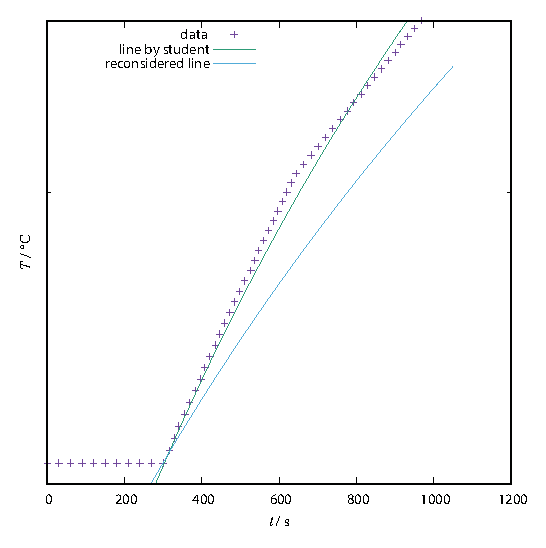
\includegraphics[scale=0.8]{hcap.eps}
 \caption{水の加熱データのプロット.下側の線が文献値に近い値を与える傾きの直線.}
 %\ecaption{Options of documentclass.}
 \label{hcap-plt}
\end{center}
\end{figure}

%\vspace{3mm}
\newpage

%%%%%%%%%%%%%%%%%%%%%%%%%%%%%%%%%%%%%%%%%%%%%%%%%%%%%%%%%%%%%%%%%%%%%%
\section{その他}
このファイルでは画像はeps形式のファイルを使っていますが,png等の画像を直接
貼り付けることも可能です.次のようにします.
\begin{verbatim}
\begin{figure}[ht]
\begin{center}
 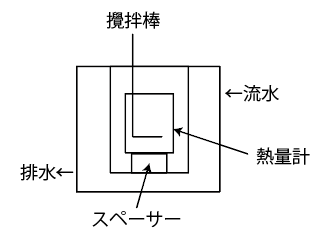
\includegraphics[scale=0.6]{aparatus2.png}
 \caption{実験装置の概略図}
 \label{apara}
\end{center}
\end{figure}
\end{verbatim}

%%%%%%%%%%%%%%%%%%%%%%%%%%%%%%%%%%%%%%%%%%%%%%%%%%%%%%%%%%%%%%%%%%%%%%
\end{document}

\begin{figure}[ht]
\begin{center}
 \includegraphics[scale=0.5]{ファイル名}
 \caption{タイトル}
 %\ecaption{Options of documentclass.}
 \label{apara}
\end{center}
\end{figure}

\begin{table}[ht]
\begin{center}
\caption{タイトル}
\label{tab1}
\begin{tabular}{ll}\hline
col1 & col2 \\ \hline
val1 & val2 \\
val3 & val4 \\ \hline
\end{tabular}%
\end{center}
\end{table}
